
Como se indica al principio del presente informe, el edificio se encuentra ubicado en Antofagasta, esto indica según la norma NCh 433 que la zona sísmica es 3. Además, al ser un edificio habitacional, se encuentra en la categoría de importancia II. También, según los antecedentes del terreno, se encuentra en un suelo tipo A. Al aplicar la norma, se determinan los siguientes parámetros sísmicos:

\begin{table}[h]
        \centering
        \begin{tabular}{|l|c|}
            \hline
            \textbf{Parámetro} & \textbf{Valor} \\
            \hline
            S & 0.9 \\
            \hline
            $T_{0}$ & 0.15s \\
            \hline
            $T'$ & 0.2s \\
            \hline
            n & 1.0 \\
            \hline
            p & 2 \\
            \hline
            $A_0$ & 0.4g \\
            \hline
            I & 1.0 \\
            \hline
            R & 1 \\
            \hline
        \end{tabular}
        \caption{Parámetros sísmicos según NCh 433}
        \label{tab:parametros_sismicos}
\end{table}

Con esta información, se puede proceder a calcular el espectro de diseño sísmico para el edificio, lo que permitirá determinar las fuerzas sísmicas que actuaran sobre la estructura y diseñar adecuadamente los elementos estructurales para resistir dichas fuerzas.

\begin{figure}[H]
    \centering
    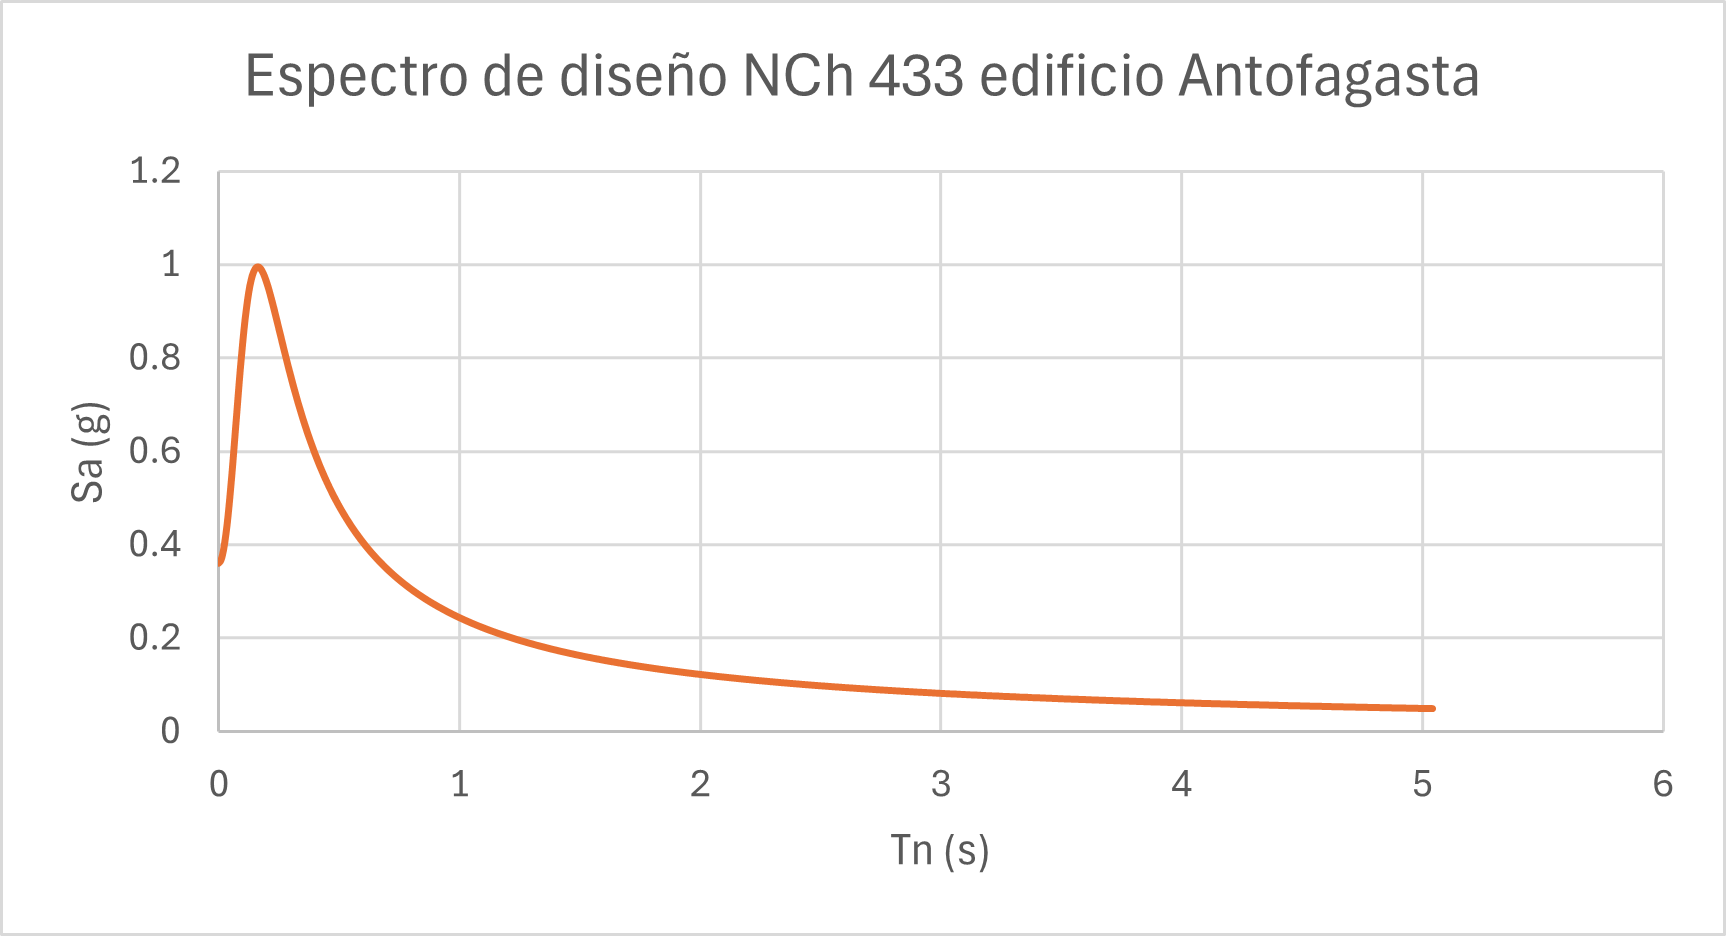
\includegraphics[width=0.8\textwidth]{secciones_inf/IMG/Espectro.png}
    \caption{Espectro de diseño sísmico para el edificio según NCh 433}
    \label{fig:espectro_sismico}
\end{figure}
